\documentclass[a4paper,12pt,obeyspaces,spaces,hyphens]{article}

\usepackage{agenda}
\usepackage{colortbl}
\usepackage{xcolor}
\usepackage{palatino}
\usepackage{calc}

\hypersetup{pdftitle={Buildroot training},
  pdfauthor={Free Electrons}}

\begin{document}

\thispagestyle{fancy}

\setlength{\arrayrulewidth}{0.8pt}

\begin{center}
\LARGE
Buildroot training\\
\large
3-day session
\end{center}
\vspace{1cm}

\small
\newcolumntype{g}{>{\columncolor{fedarkblue}}m{4cm}}
\newcolumntype{h}{>{\columncolor{felightblue}}X}

\arrayrulecolor{lightgray} {
  \setlist[1]{itemsep=-5pt}
  \begin{tabularx}{\textwidth}{|g|h|}
    {\bf Title} & Buildroot training \\
    \hline

    {\bf Overview} &
    Introduction to Buildroot \par
    Toolchains in Buildroot \par
    Root filesystem construction in Buildroot \par
    Integrating new packages in Buildroot \par
    Advanced package recipe tricks \par
    Board and project support \par
    Application development with Buildroot \\
    \hline

    {\bf Duration} & {\bf Three} days - 24 hours (8 hours per day).
    \newline 40\% of lectures, 60\% of practical labs. \\
    \hline

    {\bf Trainer} & {\bf Thomas Petazzoni}. Thomas is a major
    Buildroot developer 2009, with more than 1600 patches integrated
    and an active
    participation to the development process.\\
    \hline

    {\bf Language} & Oral lectures: English, French.
    \newline Materials: English.\\
    \hline

    {\bf Audience} & Companies interested in using Buildroot to build
    their
    embedded Linux system.\\
    \hline

    {\bf Prerequisites} & {\bf Knowledge of embedded Linux} as covered
    in our embedded Linux training
    (\url{http://free-electrons.com/training/embedded-linux/}) \newline 
    {\bf Knowledge and practice of Unix or GNU/Linux commands}
    \newline People lacking experience on this topic should get
    trained by themselves with our freely available on-line slides
    (\url{http://free-electrons.com/docs/command-line/}) \\
    \hline

    {\bf Required equipment} &
    {\bf For on-site sessions only.}
    \newline Everything is supplied by Free Electrons in public
    sessions.
    \begin{itemize}
    \item Video projector
    \item PC computers with at least 2 GB of RAM, and Ubuntu Linux
    installed in a {\bf free partition of at least 20 GB. Using Linux
      in a virtual machine is not supported}, because of issues
    connecting to real hardware.
    \item We need Ubuntu Desktop 12.04 (32 or 64 bit, Xubuntu and
    Kubuntu variants are fine). We don't support other
    distributions, because we can't test all possible package versions.
    \item {\bf Connection to the Internet} (direct or through the
    company proxy).
    \item {\bf PC computers with valuable data must be backed up}
    before being used in our sessions.  Some people have already made
    mistakes during our sessions and damaged work data.
    \end{itemize} \\
    \hline

    {\bf Materials} & Print and electronic copies of presentations and
    labs.
    \newline Electronic copy of lab files.\\
    \hline

\end{tabularx}}

\feagendatwocolumn
{Hardware}
{
  The hardware platform used for the practical labs of this training
  session is the {\bf BeagleBone Black}, which features:

  \begin{itemize}
  \item An ARM AM335x processor from Texas Instruments (Cortex-A8
    based), 3D acceleration, etc.
  \item 512 MB of RAM
  \item 2 GB of on-board eMMC storage
  	\newline(4 GB in Rev C)
  \item USB host and device
  \item HDMI output
  \item 2 x 46 pins headers, to access UARTs, SPI buses, I2C buses
    and more.
  \end{itemize}
}
{}
{
  \begin{center}
    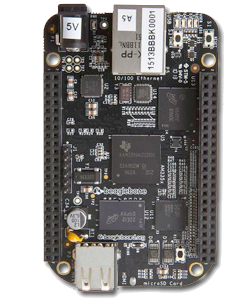
\includegraphics[height=5cm]{agenda/beagleboneblack.png}
  \end{center}
}

\section{Day 1 - Morning}

\feagendatwocolumn
{Lecture - Embedded Linux and build system introduction}
{
  \begin{itemize}
  \item The general architecture of an embedded Linux system
  \item Build systems vs. binary distributions
  \item Comparaison of existing build systems
  \end{itemize}
}
{Lecture - Introduction to Buildroot}
{
  \begin{itemize}
  \item Buildroot project organization
  \item Basic configuration and usage of Buildroot
  \end{itemize}
}
\\
\feagendatwocolumn
{Lab - Basic Buildroot usage}
{
  \begin{itemize}
  \item Getting and setting up Buildroot
  \item Configuring a basic system with Buildroot
  \item Running the system on a hardware platform and in the Qemu
    emulator, with the root filesystem over NFS or the root filesystem
    flashed
  \end{itemize}
}
{Lecture - Buildroot source and build trees}
{
  \begin{itemize}
  \item Details about the Buildroot source code organization
  \item Details about the Buildroot build tree
  \end{itemize}
}

\section{Day 1 - Afternoon}

\feagendatwocolumn
{Lecture - Toolchains in Buildroot}
{
  \begin{itemize}
  \item The different choices for using toolchains in Buildroot
  \item Using existing binary toolchains, such as Sourcery CodeBench
    toolchains, understanding {\em multilib} capabilities and
    integration of toolchains in Buildroot
  \item Generating custom toolchains with Buildroot and {\em Crosstool-ng}
  \item Details on using and configuring {\em Crosstool-ng}
  \end{itemize}
}
{Lab - Toolchains in Buildroot}
{
  \begin{itemize}
  \item Explore the integration of external toolchains in Buildroot
    and test the {\em multilib} mechanism with Sourcery CodeBench
    toolchains
  \item Use {\em Crosstool-NG} to generate a custom toolchain, and
    integrate it into Buildroot
  \end{itemize}
}

\section{Day 2 - Morning}

\feagendatwocolumn
{Lecture - Root filesystem construction in Buildroot}
{
  \begin{itemize}
  \item Understand how Buildroot builds the root filesystem: {\em
      skeleton} and installation of packages
  \item Customization of the root filesystem contents
  \item Understand the configuration of the {\em console}
  \item Study the different options for managing the {\tt /dev}
    directory: static or dynamic, with mdev or udev
  \item Understand how Buildroot generates filesystem images
  \end{itemize}
}
{Lab - Root filesystem construction}
{
  \begin{itemize}
  \item Generate Buildroot systems with different {\tt /dev}
    management options and test them on an hardware platform.
  \item Customize the root filesystem contents
  \end{itemize}
}
\\
\feagendaonecolumn
{Lecture - Integrating new packages in Buildroot}
{
  \begin{itemize}
  \item How to integrate new packages in the Buildroot configuration
    system
  \item Understand the different package infrastructures (for {\em
      generic} packages, {\em autotools} packages, {\em CMake}
    packages and {\em Python} packages)
  \item Details on writing a package recipe: describing the package
    source code location, download method, configuration, build and
    installation steps, handling dependencies, etc.
  \end{itemize}
}

\section{Day 2 - Afternoon}

\feagendatwocolumn
{Lab - New packages in Buildroot}
{
  \begin{itemize}
  \item Practical creation of several new packages in Buildroot,
    using the different package infrastructures.
  \end{itemize}
}
{Lecture - Advanced package recipe tricks}
{
  \begin{itemize}
  \item Understanding {\em hooks}
  \item Packaging software available from the local filesystem ({\em
      local} and {\em file} fetching methods)
  \item Best practices to use packages during development of
    applications and libraries ({\em source override} mechanism)
  \end{itemize}
}
\\
\feagendaonecolumn
{Lab - Advanced package recipe tricks}
{
  \begin{itemize}
  \item Use {\em hooks} in packages
  \item Use special features for custom software
  \end{itemize}
}

\section{Day 3 - Morning}

\feagendatwocolumn
{Lecture - Board and project support}
{
  \begin{itemize}
  \item Understand how to handle board-specific and project-specific
    information
  \item Storing the kernel and bootloader configuration and patches
  \item Storing the project configuration
  \item Handling root filesystem customization (post-build script,
    skeleton, etc.)
  \item How to version control project-specific changes
  \end{itemize}
}
{Lab - Board and project support}
{
  \begin{itemize}
  \item Create a Buildroot configuration for a specific project, with:
    \begin{itemize}
    \item a custom kernel configuration
    \item custom packages
    \item special root filesystem modifications.
    \end{itemize}
  \end{itemize}
}

\section{Day 3 - Afternoon}

\feagendatwocolumn
{Lecture - Application development with Buildroot}
{
  \begin{itemize}
  \item Using Buildroot during application development
  \item Usage of the Buildroot environment to build applications
    outside of Buildroot
  \item Generate an SDK for other developers
  \item Remote debugging with Buildroot
  \end{itemize}
}
{Lab - Application development with Buildroot}
{
  \begin{itemize}
  \item Experiment application development and debugging with
    Buildroot, through a practical example on our target system.
  \item Setting up an Eclipse-based development environment, using the
    Buildroot Eclipse plugin.
  \end{itemize}
}
\\
\feagendatwocolumn
{Lecture - Understanding Buildroot internals}
{
  \begin{itemize}
  \item Detailed description of the Buildroot build process:
    toolchain, packages, root filesystem construction, stamp files,
    etc.
  \item Understanding virtual packages.
  \end{itemize}
}
{Lecture - Getting support and contributing}
{
  \begin{itemize}
  \item Getting support: {\em bugzilla}, {\em mailing list}, {\em IRC}
  \item Contributing: understanding the development process, how to
    submit patches
  \end{itemize}
}

\end{document}
